\documentclass[11pt]{book}
\usepackage[reqno]{amsmath} % Paquete para el manejo de expresiones matemáticas [reqno], [leqno] y [fleqn]
\usepackage{amsthm}
\usepackage{amssymb,amsmath,latexsym} %Paquete para llamar símbolos matemáticos
\usepackage{amsfonts}
\usepackage[mathscr]{euscript}
\usepackage{graphicx} %paquete para el manejo de transformaciones geométricas de imagénes
\usepackage{color} %paquete para el manejo de color en textos.
%\usepackage[utf8]{inputenc} %paquete para el manejo de caracteres acentuados
\usepackage[french,spanish]{babel} %paquete que genera documentos en diferentes idiomas
\usepackage{enumerate}
\usepackage{multicol} % Paquete para modificar el número de columnas
\usepackage{layout} % Paquete  para revisar los valores de 
\usepackage{verbatim}
\pagestyle{myheadings}  % Estilo de página
%\pagenumbering{arabic} % Estilo de numéración
\hoffset1cm
\newcounter{Teorema}
\newcommand{\Teorema}{\stepcounter{Teorema}{\bf Teorema \theTeorema.} }
\usepackage{ tipa }



\DeclareMathOperator{\arcsec}{arcsec} % Creación de nuevos comandos en latex
\DeclareMathOperator{\Var}{Var}

\DeclareMathOperator*{\Hom}{Hom}

\setcounter{MaxMatrixCols}{15}

\allowdisplaybreaks % Control de cambios de página en alineaciones

\decimalpoint

%\renewcommand{\theequation}{\thesection.\arabic{equation}}
\numberwithin{equation}{section}
%\renewcommand{\theequation}{\theparentequation\arabic{equation}}


%% Nuevos teoremas

\theoremstyle{plain}  % Requiere el paquete amsthm

\newtheorem{thm}{Teorema}[section]
\newtheorem{Corol}[thm]{Colorario}
\newtheorem{Prop}[thm]{Proposición}
\newtheorem{axiom[thm]}{Axioma}
\newtheorem{conj}{Conjetura}
\newtheorem{Def}{Definición}[section]
\newtheorem{Ej}{Ejemplo}[section]
\newtheorem{notacion}[Def]{Notación}
\newtheorem{nota}[Def]{Nota}

%\renewcommand{\qedsymbol}{$\heartsuit$}
\providecommand{\abs}[1]{\lvert#1\rvert} %valor absoluto
\providecommand{\norm}[1]{\lVert#1\rVert} %norma
\pagestyle{empty}



\begin{document}

\section{Grupos continuos}
La teoría de los grupos continuos fue creada por el matemático noruego Sophus Lie en la 
década de 1870. Inicialmente, su objetivo era desarrollar una teoría de ecuaciones
diferenciales como la teoría de ecuaciones polinómicas de Galois. Vio que cada 
ecuación diferencial tiene un grupo, análogo al grupo de Galois pero “continuo”
en lugar de finito, y que los grupos “simples” presentan un obstáculo para la 
solución. 
\\
\textbf{
Así, su atención se desplazó rápidamente al problema de clasificar 
grupos continuos y (particularmente) identificar los grupos simples entre ellos. 
La definición de un "grupo continuo", o lo que ahora llamamos un grupo de Lie, 
es algo sutil, como lo es la definición de "simple" para estos grupos. 
Aquí nos contentamos simplemente con dar algunos ejemplos y probar la simplicidad 
de uno de ellos.}
\\
El ejemplo más fácil de entender de un grupo continuo es la recta numérica R, bajo 
la operación de suma. Este grupo es “continuo” en el sentido de que la operación de grupo $x , y \to x+y$, y también la operación inversal de grupo $x \to -x$, es una 

función continua. Un ejemplo relacionado es el círculo unitario


\begin{equation*}
    \mathbb{S}^{1}=\{z : \abs{z}=1\}
\end{equation*}

en el plano de los números complejos, bajo la operación
(obviamente continua) de multiplicación de números complejos.
$\mathbb{S}^{1}$ también se llama SO(2), el primero de una familia llamada 
especiales ortogonales o de rotación. Podemos interpretar un 
miembro z de SO(2) como una rotación del plano, porque
\begin{equation*}
    z = \cos{\theta}+ i \sin{\theta}\text{, para algun } \theta
\end{equation*}
y multiplicando cada número complejo por z gira el plano $\mathbb{C}$
alrededor de $O$ a través del ángulo $\theta$. Por lo tanto, la operación
de grupo en $SO(2)$ también puede verse como una suma de ángulos,
que es otra forma de ver que $SO(2)$ es continua. Tanto $\mathbb{R}$ y
$SO(2)$ son grupos abelianos, por lo que no son muy interesantes. 
El primer grupo continuo realmente interesante es $SO(3)$, el
grupo de rotación del espacio tridimensional $\mathbb{R}^{3}$. Si tomamos
una rotación $r$ de $\mathbb{R}^{3}$ dada por un eje $A$ que pasa por $O$ y un
giro de ángulo $\theta$ alrededor de $A$, entonces ni siquiera es obvio
que las rotaciones espaciales formen un grupo. Dada una
rotación $r$ con eje $A$ y ángulo $\theta$, y una rotación $s$ con eje $B$ 
ángulo $\varpi$, ¿podemos estar seguros de que la combinación $sr$ tiene
incluso un eje $C$ y un ángulo $X$ bien definidos? La 
(sí) aparentemente fue encontrada por primera vez por Euler
(1776), pero ahora podemos encontrar esta respuesta mucho más
fácilmente. El truco consiste en ver cada rotación como un
producto de dos reflexiones, como se muestra en la figura 1.

La imagen de la izquierda en la figura muestra un par de líneas en el plano, 
$L$ y $M$, que se encuentran en $O$ en el ángulo $\theta/2$. Si
un punto $X$ se refleja en $L$ (hacia $X'$), entonces en $M$ (hacia $X''$),
el ángulo entre $X$ y $X''$ es claramente $\theta$. De manera más general,
está claro que una rotación alrededor de cualquier punto $Y$ a
través del ángulo $\theta$ puede realizarse mediante reflexiones
sucesivas en dos líneas cualesquiera a través de $Y$ que se
encuentran en el ángulo $\theta/2$ (medido en el sentido apropiado).
Lo mismo es cierto para la rotación de una esfera, y por tanto
de $\mathbb{R}^{3}$ , alrededor de cualquier eje. 
Para rotar a través del
ángulo $\theta$ alrededor del eje $YY'$ (imagen de la derecha) basta con
reflejar en dos grandes círculos cualesquiera a través de $Y$ e $Y'$
que se encuentran en el ángulo $\theta/2$. De manera equivalente, uno
refleja la esfera en cualquiera de los dos planos que se
encuentran a lo largo de la línea $YY'$ en el ángulo $\theta/2$.

\begin{figure}[h]
\centering
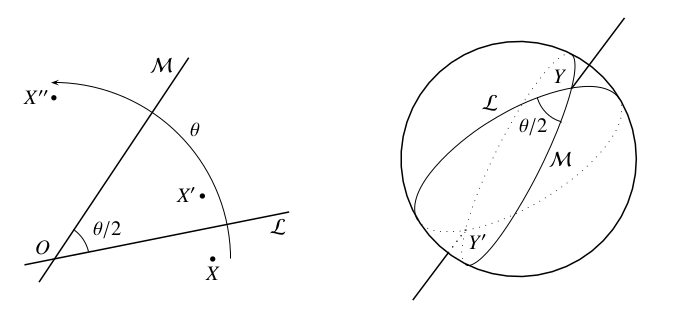
\includegraphics[scale=0.5]{imagenes/23.3-1.png}
\caption{Rotación a través de un par de reflexiones}
\end{figure}

Supongamos ahora que queremos encontrar el resultado de
realizar la rotación $r$ de la esfera, con eje que pasa por $P$ y
ángulo $\theta$, luego la rotación $s$ con eje
a través de $Q$ y el ángulo $\varphi$. Haciendo uso de nuestra
libertad para elegir los grandes círculos de reflexión,
realizamos $r$ por el par de reflexiones en los grandes
círculos $L$ y $M$ a través de $P$ que están separados por un ángulo $\theta/2$, donde $M$ pasa a través de $P$ y $Q$ (Figura 2).)

\newpage
\begin{figure}[h]
\centering
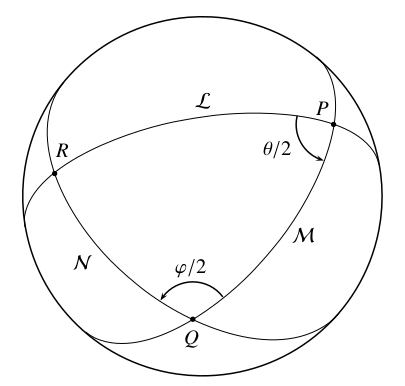
\includegraphics[scale=0.5]{imagenes/23.3-2.png}
\caption{Hallar el producto de rotaciones}
\end{figure}

Luego nos damos cuenta de $s$ por el par de reflexiones en $M$ y $N$ a través de $Q$ que están separadas por un ángulo $\varphi/2$. De ello se deduce, dado que las reflexiones sucesivas en $M$ se cancelan, asi

\begin{center}
    $sr$ = reflejo en $L$ luego reflejo en $M$ luego reflejo en $M$ luego reflejo en $N$ \\
    = reflexión en $L$ luego reflexión en $N$ \\
    = rotación alrededor del eje RR a través del ángulo $x$,
\end{center}
donde $R$ es el tercer vértice y $x/2$ es el tercer ángulo, en el
triángulo esférico formado por los grandes círculos $L$, $M$ y $N$.
Así, el producto de las rotaciones es una rotación. Como
siempre, esta operación de “producto” es asociativa, porque es
el producto de funciones. También es claro que la inversa de
una rotación es una rotación (mismo eje, negativo del ángulo),
por lo que las rotaciones forman un grupo bajo la operación
producto. Finalmente, es intuitivamente claro que el producto y
el inverso dependen continuamente de la posición del eje y del
ángulo de rotación. Entonces este grupo $SO(3)$ es continuo. En
la siguiente sección veremos que la continuidad es crucial para
demostrar que $SO(3)$ es un grupo simple.

\section{Simplicidad de $SO(3)$}

Para demostrar que $SO$ es simple, consideramos un subgrupo
normal $H \not = {1}$ y pretendemos demostrar que $H = SO(3)$. Como $H$ es
normal, $gH = Hg$, 
y por lo tanto $gHg^{-1} = H$
para cada $g$ en
$SO(3)$. 
En otras palabras, 
$gHg^{-1}$ está en $H$ para
cada $g$ en $SO(3)$
y cada $h$ en $H$. Esto nos permite construir muchos elementos de $H$
a partir de un elemento no trivial $h$ y, de hecho, podemos
construir todos los elementos de $SO( 3)$. Los construimos en
tres pasos, comenzando con una $h$ específica con eje $A$ y ángulo
$\theta$ distinto de cero:
\begin{itemize}
    \item[\textbf{step 1.}] H incluye la rotación a través del ángulo $\theta$ sobre cualquier eje B. \\ 
    Para ver por qué, sea g una rotación que mueve el eje A al eje B. Entonces $gHg^{-1}$ es la rotación a través del ángulo $\theta$ alrededor del eje $B$ porque
    \begin{itemize}
        \item $g^{-1}$ mueve el eje $B$ a la posición del eje $A$.
        \item $h$ gira $\mathbb{R}^{3}$ sobre el eje $A$ a través del ángulo $\theta$.
        \item $g$ mueve el eje en la posición $A$ de regreso a su posición original $B$.
    \end{itemize} 
    \item[\textbf{Step 2}] $H$ incluye rotaciones a través de todos los ángulos en un intervalo entre algunos $\alpha$ y $\beta$, $\alpha$ < $\beta$.
    Como sabemos de la sección anterior, el producto de 
    rotación r alrededor del eje PP a través del ángulo $\theta$ y una
    rotación s alrededor del eje $QQ'$ a través del ángulo $\theta$ es
    una rotación alrededor del eje $RR'$ a través del ángulo $X$,
    donde $R$ y $X/2$ son como se muestra en Figura 3.
    
    \begin{figure}[h]
\centering
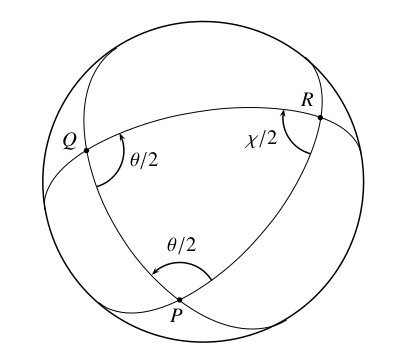
\includegraphics[scale=0.5]{imagenes/23.4.png}
\caption{Hallar el producto de rotaciones}
\end{figure}

Supongamos ahora que $P$ es fijo y que se permite que $Q$ varíe
continuamente a lo largo de un gran círculo fijo que pasa por
$P$. Cuando $Q$ está cerca de $P$, también lo está $R$; por tanto, 
triángulo $PQR$ es casi euclidiano y la suma de sus ángulos es
cercana a $\pi$. 
De ello se deduce que $X/2$ está 
cerca de 
$\pi - \theta$.
A medida que $P$ se aleja, el triángulo esférico $PQR$ se vuelve más
grande, por lo que también lo hace la suma de sus ángulos según
la Sección 17.6, por lo que $X/2$ se vuelve más grande. Dado que
$X/2$ varía continuamente con la posición de $Q$, necesariamente
toma todos los valores en un intervalo entre algún $\alpha$ y $\beta$, donde $\alpha < \beta$ 



\item[\textbf{Step 3.}] $H$ incluye rotaciones a través de cualquier ángulo.
\\
Como $\alpha < \beta$, el intervalo entre $\alpha$ y $\beta$ incluye un subintervalo
de la forma $[2m\pi / n, 2(m+1)\pi / n]$, para algunos enteros $m$ y $n$.
Por tanto, del Paso 2 y el Paso 1 se deduce que $H$ incluye
todas las rotaciones, alrededor de un eje fijo $B$, con ángulos
entre $2m\pi / n$ y $2(m+1)\pi /n$. Por supuesto, $H$ también incluye
todos los productos de sus miembros y, por lo tanto, todas
sus n-ésimas potencias, que multiplican los ángulos por $n$.
Pero si multiplicamos los ángulos entre $2m\pi /n$ y $2(m + 1)\pi /n$
por $n$, obtenemos todos los ángulos, según sea necesario.
\\
Aplicando el Paso 1 nuevamente, obtenemos rotaciones con
todos los ángulos y todos los ejes, por lo que $H$ incluye
todos los elementos de $SO(3)$, como se afirma. Lie observó la
simplicidad de muchos grupos de Lie, incluido $SO(3)$, pero sus
conceptos de  \textquoteleft grupo \textquoteright y \textquoteleft simplicidad \textquoteright eran algo diferentes a
los nuestros. En su opinión, un \textquoteleft grupo \textquoteright incluía \textquoteleft elementos
\textquoteleft infinitesimales\textquoteright, y los usó para determinar la simplicidad.
Hoy, llamamos a los \textquoteleft elementos infinitesimales \textquoteright de un grupo
de Lie sus vectores tangentes en la identidad, y construimos
a partir de ellos una estructura algebraica separada llamada
álgebra de Lie del grupo de Lie. Un álgebra de Lie tiene una
operación de \textquoteleft producto\textquoteright , llamada paréntesis de Lie, que es
bastante diferente de una operación de grupo; por ejemplo, el
corchete de mentira no es asociativo. Sin embargo, es una
buena idea mirar las álgebras de Lie. Existe un concepto
natural de simplicidad para las álgebras de Lie, de modo que
un grupo de Lie simple tiene un álgebra de Lie simple, y
probar la simplicidad es algo más fácil para las álgebras que
para los grupos. La desventaja, si la hay, es que un álgebra
de Lie simple puede no provenir de un grupo de Lie simple.
\\


Por ejemplo, el grupo $SU(2)$ del conjunto de ejercicios
anterior tiene el mismo álgebra de Lie que $SO(3)$, por lo que
el álgebra de Lie de $SU(2)$ es simple. Sin embargo, el grupo
$SU(2)$ no es simple; tiene un subgrupo normal con los
elementos 
1 y -1.
El problema es que el álgebra de Lie no
puede "detectar" los elementos del grupo que están lejos del
elemento de identidad, por lo que puede pasar por alto un
subgrupo normal cuyos miembros que no son de identidad están
todos lejos (como es el caso de $SU(2))$. Esto no es
necesariamente algo malo y, de hecho, muchos autores definen
un grupo de Lie como simple si su álgebra de Lie es simple.

\end{itemize}
\end{document}